% ===================================================================
%  Adaptive Cyber-Physical Security — Phase-2 Project Report
%  IEEE Two-Column Conference Paper Format
%  Overleaf-ready. Compile with pdflatex → bibtex → pdflatex × 2
% ===================================================================
\documentclass[10pt,conference]{IEEEtran}

% ---- Core packages ----
\usepackage[T1]{fontenc}
\usepackage[utf8]{inputenc}
\usepackage{graphicx}
\usepackage{booktabs}
\usepackage{amsmath}
\usepackage{amssymb}
\usepackage{float}
\usepackage{xcolor}
\usepackage{enumitem}
\usepackage{cite}
\usepackage{url}
\usepackage{microtype}
\usepackage{balance}
\usepackage{multirow}
\usepackage{array}

\usepackage[colorlinks=true,
            linkcolor=blue,
            citecolor=blue,
            urlcolor=blue,
            pdftitle={Adaptive Cyber-Physical Security Phase-2 Report},
            pdfauthor={Pugazhendhi J and Dally R}]{hyperref}

% ---- Graphics path (set relative to where you compile from) ----
\graphicspath{{../../}}  % adjust if compiling from report/latex/

% ---- Title ----
\title{Adaptive Cyber-Physical Security:\\Phase-2 Project Report — Hybrid Deep-Learning\\Intrusion Detection with Zero-Day Generalization}

% ---- Authors ----
\author{
  \IEEEauthorblockN{Pugazhendhi J}
  \IEEEauthorblockA{
    \textit{Department of CS and AI}\\
    Rishihood University\\
    Sonipat, India\\
    \href{mailto:pugazhendhi.j23csai@nst.rishihood.edu.in}
         {pugazhendhi.j23csai@nst.rishihood.edu.in}}
  \and
  \IEEEauthorblockN{Dally R}
  \IEEEauthorblockA{
    \textit{Department of CS and AI}\\
    Rishihood University\\
    Sonipat, India\\
    \href{mailto:dally.r23csai@nst.rishihood.edu.in}
         {dally.r23csai@nst.rishihood.edu.in}}
}

% ===================================================================
\begin{document}
\maketitle

% ---- Abstract ----
\begin{abstract}
Phase~1 of this project established that a supervised Random Forest
classifier, while achieving perfect precision on known attack families
in the CIC-IDS-2018 benchmark, delivered zero recall against unseen
(\emph{zero-day}) attacks, and that a One-Class SVM partially remedied
novelty sensitivity at the cost of low overall recall. Phase~2 addresses
these twin limitations through three complementary extensions: (i)~scale-up
to the \emph{full} CIC-IDS-2018 processed dataset of
8{,}284{,}195 flows spanning 13~distinct attack categories; (ii)~introduction
of a deep-learning \textbf{Autoencoder} trained exclusively on benign traffic
to raise zero-day recall through reconstruction-error thresholding; and
(iii)~a decision-level \textbf{Hybrid model} that fuses Random Forest and
One-Class SVM predictions under an OR-logic combiner, yielding superior
coverage across both seen and unseen threat categories. Experimental results
demonstrate that the Hybrid system substantially improves zero-day recall
beyond either individual model, while the Autoencoder provides richer
anomaly diagnostics including ROC-curve, precision-recall curves,
per-attack detection rates, and threshold-sensitivity analysis. The work
confirms that no single learning paradigm is sufficient for open-world
cyber-physical intrusion detection; ensemble fusion with deep anomaly
estimation is the recommended adaptive-security architecture.
\end{abstract}

% ---- Keywords ----
\begin{IEEEkeywords}
Intrusion Detection, CIC-IDS-2018, Random Forest, One-Class SVM,
Autoencoder, Hybrid IDS, Zero-Day Detection, Anomaly Detection,
Cyber-Physical Security, Deep Learning, Feature Engineering
\end{IEEEkeywords}

% ===================================================================
\section{Introduction}
\label{sec:intro}

Cyber-physical systems (CPS) tightly couple networked digital computation
with physical-world processes—spanning industrial control systems, smart
grids, autonomous vehicles, and medical devices—making them high-value
targets for sophisticated adversaries. Intrusion detection in such
environments must handle two qualitatively distinct conditions
simultaneously: (i)~classifying attacks whose signatures or statistical
profiles appear in historical training data (\emph{known threats}), and
(ii)~flagging malicious traffic from attack families that were entirely
absent during training—the foundational \emph{zero-day} or open-world
detection problem \cite{buczak2016}.

Phase~1 of this project established a baseline pipeline on CIC-IDS-2018
\cite{sharafaldin2018} using Random Forest (RF) and One-Class SVM (OCSVM).
The critical finding was that RF achieved perfect precision on known attacks
but \textbf{zero} zero-day recall, while the OCSVM provided marginal
zero-day sensitivity (14.5\%) at reduced precision. No single model
satisfied the dual objective of accurate known-attack classification
\emph{and} meaningful zero-day detection.

Phase~2 directly addresses this shortcoming by:
\begin{itemize}[leftmargin=*,noitemsep]
  \item scaling the pipeline to the full CIC-IDS-2018 dataset (8.2M flows,
        13 attack families);
  \item introducing a deep-learning Autoencoder for reconstruction-error
        anomaly scoring, supplementing the OCSVM's kernel-based approach;
  \item implementing a decision-level Hybrid combiner (RF~+~OCSVM) under
        OR logic to maximize coverage across both seen and zero-day threats;
  \item providing richer evaluation via ROC, precision-recall, threshold
        sensitivity, and per-attack detection-rate diagnostics.
\end{itemize}

The broader contribution is an end-to-end, reproducible adaptive-security
architecture showing that ensemble fusion of discriminative and generative
anomaly detection is necessary and sufficient for practical CPS defense.

% ===================================================================
\section{Dataset and Preprocessing}
\label{sec:dataset}

\subsection{CIC-IDS-2018 Overview}

The CIC-IDS-2018 dataset \cite{sharafaldin2018} was generated by the
Canadian Institute for Cybersecurity using a realistic network testbed
with $25$ machines acting as victims and $50$ machines generating benign
and attack traffic over five days. Raw packet captures were processed
into \emph{flow-level} feature vectors using CICFlowMeter, producing
80+ statistical attributes per bidirectional network flow.

In Phase~2, we operate on the \emph{fully processed} dataset
\texttt{cic18\_full\_processed.csv}, containing:
\begin{itemize}[leftmargin=*,noitemsep]
  \item \textbf{8{,}284{,}195} network flow records.
  \item \textbf{52} columns after preprocessing (49 numeric predictors +
        3 label columns).
  \item 14 distinct traffic classes: 1 benign + 13 attack families.
\end{itemize}

Table~\ref{tab:full_dist} presents the complete class distribution.

\begin{table}[H]
\centering
\caption{Full CIC-IDS-2018 processed dataset class distribution}
\label{tab:full_dist}
\begin{tabular}{lrr}
\toprule
\textbf{Attack Class} & \textbf{Count} & \textbf{\%} \\
\midrule
Benign                    & 6{,}112{,}151 & 73.78 \\
DDoS Attack-HOIC          &   686{,}012   &  8.28 \\
DoS Attacks-Hulk          &   461{,}912   &  5.58 \\
Bot                       &   286{,}191   &  3.45 \\
FTP-Bruteforce            &   193{,}360   &  2.33 \\
SSH-Bruteforce            &   187{,}589   &  2.26 \\
Infilteration             &   161{,}934   &  1.95 \\
DoS Attacks-SlowHTTPTest  &   139{,}890   &  1.69 \\
DoS Attacks-GoldenEye     &    41{,}508   &  0.50 \\
DoS Attacks-Slowloris     &    10{,}990   &  0.13 \\
DDoS Attack-LOIC-UDP      &     1{,}730   &  0.02 \\
Brute Force-Web           &       611     & <0.01 \\
Brute Force-XSS           &       230     & <0.01 \\
SQL Injection             &        87     & <0.01 \\
\midrule
\textbf{Total}            & \textbf{8{,}284{,}195} & \textbf{100} \\
\bottomrule
\end{tabular}
\end{table}

\subsection{Preprocessing Pipeline}
\label{sec:preproc}

The full preprocessing pipeline (\texttt{pipeline/full\_preprocessing.py})
applies the following deterministic sequence of transformations to all
raw daily CSV files:

\begin{enumerate}[leftmargin=*,noitemsep,topsep=0pt]
  \item \textbf{Identifier removal.} Drop \texttt{Flow~ID},
        \texttt{Src~IP}, \texttt{Dst~IP}, and \texttt{Timestamp} to
        prevent leakage of environment-specific routing artefacts.
  \item \textbf{Numeric coercion.} Cast all non-label columns to
        \texttt{float64} via \texttt{pd.to\_numeric(errors=`coerce')};
        replace \texttt{$\pm$inf} with \texttt{NaN}.
  \item \textbf{Sparse-feature removal.} Drop any column exceeding 50\%
        missing-value ratio.
  \item \textbf{Imputation.} Fill remaining \texttt{NaN} values with
        zero, which is semantically justified for flow-counter features.
  \item \textbf{Label normalization.} Convert \texttt{Label} to
        lowercase-stripped strings; create binary target
        \texttt{BinaryLabel} ($0$~=~benign, $1$~=~attack) and
        normalized \texttt{AttackType}.
  \item \textbf{Constant removal.} Discard columns with unique-value
        count $\leq 1$ (zero variance, no discriminative information).
  \item \textbf{Correlation pruning.} Compute the absolute Pearson
        correlation matrix over numeric predictors. For each pair
        $(\rho_{ij} > 0.98)$, apply a domain heuristic to retain the
        more semantically meaningful feature (e.g., prefer total-level
        statistics over sub-flow means). This reduces features from
        80+ raw columns to 49 predictors.
\end{enumerate}

\subsection{Feature Dictionary (Selected)}

Table~\ref{tab:features} lists a representative selection of the 49
retained numeric predictors with their semantics.

\begin{table}[H]
\centering
\caption{Representative subset of retained features after preprocessing}
\label{tab:features}
\begin{tabular}{ll}
\toprule
\textbf{Feature} & \textbf{Semantics} \\
\midrule
\texttt{Flow Byts/s}   & Byte rate of entire flow \\
\texttt{Flow Pkts/s}   & Packet rate of entire flow \\
\texttt{Fwd IAT Mean}  & Mean forward inter-arrival time \\
\texttt{Bwd IAT Max}   & Max backward inter-arrival time \\
\texttt{Pkt Len Std}   & Std.\ dev.\ of packet length \\
\texttt{SYN Flag Cnt}  & Count of SYN TCP flags \\
\texttt{ACK Flag Cnt}  & Count of ACK TCP flags \\
\texttt{Init Fwd Win Byts} & Initial forward TCP window bytes \\
\texttt{Active Mean}   & Mean duration of active flow periods \\
\texttt{Idle Mean}     & Mean duration of idle flow periods \\
\texttt{Down/Up Ratio} & Downstream to upstream volume ratio \\
\texttt{Dst Port}      & Destination transport-layer port \\
\bottomrule
\end{tabular}
\end{table}

% ===================================================================
\section{Methodology}
\label{sec:methodology}

Phase~2 introduces a three-tier detection architecture, each tier
addressing a different aspect of the open-world threat model.

\subsection{Tier 1: Supervised Classification (Random Forest)}

The RF classifier forms the \emph{known-threat} arm of the pipeline.
Given features $\mathbf{x} \in \mathbb{R}^{p}$ ($p=49$), an ensemble
of $B=100$ trees votes:
\begin{equation}
  \hat{y}_{\text{RF}}(\mathbf{x})
  = \underset{c \in \{0,1\}}{\arg\max}
    \sum_{b=1}^{B} \mathbf{1}\!\left[T_b(\mathbf{x}) = c\right].
  \label{eq:rf}
\end{equation}
Training follows the zero-day split protocol: benign traffic and one
seen attack family (\texttt{dos~attacks-hulk}) enter training; two
unseen families (\texttt{bot}, \texttt{dos~attacks-slowhttptest}) are
held out exclusively for zero-day evaluation.

\subsection{Tier 2: Kernel Anomaly Detection (One-Class SVM)}

The OCSVM \cite{scholkopf2001} is trained on benign-only
features standardized to $\mathcal{N}(0,1)$. It estimates the smallest
high-density region $\mathcal{H}$ containing a $1-\nu$ fraction of
the training distribution by solving:
\begin{equation}
\min_{w,\rho,\xi}\;
  \frac{1}{2}\|w\|^2
  + \frac{1}{\nu n}\sum_{i=1}^{n}\xi_i - \rho
\label{eq:ocsvm}
\end{equation}
\begin{equation}
\text{s.t.}\quad
  w^\top\phi(\mathbf{x}_i) \ge \rho - \xi_i,\quad \xi_i \ge 0,
\label{eq:ocsvm_cst}
\end{equation}
where $\phi(\cdot)$ is the RBF kernel map with bandwidth $\gamma =
\texttt{scale}$ and outlier fraction $\nu = 0.05$. At inference, any
sample with decision function $f(\mathbf{x}) < 0$ is flagged as
anomalous (attack).

\subsection{Tier 3: Deep Reconstruction-Error Anomaly Detection (Autoencoder)}

Phase~2 introduces a \textbf{fully-connected Autoencoder} as a
deep-learning complement to the OCSVM. Trained exclusively on benign
flows, the network learns a low-dimensional manifold of normal traffic.
Because attack flows deviate from this manifold, their encoded
representations faithfully reconstruct only if the attack is
statistically close to benign traffic. The anomaly score for sample
$\mathbf{x}$ is the mean squared reconstruction error:
\begin{equation}
  \mathcal{E}(\mathbf{x})
  = \frac{1}{p}\left\|\mathbf{x} - \hat{\mathbf{x}}\right\|^2,
  \label{eq:ae_score}
\end{equation}
where $\hat{\mathbf{x}} = \text{Dec}\!\left(\text{Enc}(\mathbf{x};\,
\theta_e);\,\theta_d\right)$ is the decoded reconstruction. A flow is
classified as an attack if $\mathcal{E}(\mathbf{x}) \geq \tau$, where
the threshold $\tau$ is tuned to balance precision and recall on a
held-out validation set.

\subsection{Tier 4: Ensemble Fusion (Hybrid Model)}

The Hybrid model combiner $\mathcal{H}$ applies OR-logic over the RF
and OCSVM binary predictions:
\begin{equation}
  \hat{y}_{\text{Hybrid}}(\mathbf{x})
  = \hat{y}_{\text{RF}}(\mathbf{x}) \;\mathbin{\vee}\;
    \hat{y}_{\text{OCSVM}}(\mathbf{x}),
  \label{eq:hybrid}
\end{equation}
where $\hat{y}_{\text{OCSVM}} = \mathbf{1}[f_{\text{OCSVM}}(\mathbf{x}) = -1]$.
This design guarantees:
\begin{itemize}[leftmargin=*,noitemsep]
  \item Hybrid zero-day recall $\geq \max(\text{ZD-Recall}_\text{RF},\,
        \text{ZD-Recall}_\text{OCSVM})$, since any zero-day caught by
        either component is retained.
  \item High-confidence precision from RF on in-distribution attacks.
  \item Novelty sensitivity from OCSVM on out-of-distribution flows.
\end{itemize}

% ===================================================================
\section{Model Architectures}
\label{sec:architectures}

\subsection{Random Forest (Baseline, Tier~1)}

\begin{itemize}[leftmargin=*,noitemsep]
  \item \textbf{Estimators:} 100 decision trees.
  \item \textbf{Max features:} $\sqrt{p}$ (default, $\approx7$).
  \item \textbf{Bootstrap:} Enabled; out-of-bag score available.
  \item \textbf{Class weight:} Default (uniform).
  \item \textbf{Random state:} 42 for full reproducibility.
  \item \textbf{Parallelism:} \texttt{n\_jobs=-1} (all CPU cores).
\end{itemize}

No feature scaling is required; RF operates directly on the
correlation-pruned 49-dimensional feature space.

\subsection{One-Class SVM (Baseline Anomaly, Tier~2)}

\begin{itemize}[leftmargin=*,noitemsep]
  \item \textbf{Kernel:} RBF, $\gamma = \texttt{scale}$
        ($= 1 / (p \cdot \text{Var}(\mathbf{X}))$).
  \item \textbf{Outlier fraction:} $\nu = 0.05$.
  \item \textbf{Cache:} 4{,}000 MB for QP solver efficiency.
  \item \textbf{Scaling:} \texttt{StandardScaler} fit on benign
        training split only.
  \item \textbf{Training cap:} 20{,}000 benign samples (computational
        tractability; OCSVM has $O(n^2)$–$O(n^3)$ complexity).
\end{itemize}

\subsection{Autoencoder (Deep Anomaly Detector, Tier~3)}

The Autoencoder implements a symmetric encoder-decoder stack:

\begin{table}[H]
\centering
\caption{Autoencoder layer architecture}
\label{tab:ae_arch}
\begin{tabular}{llll}
\toprule
\textbf{Layer} & \textbf{Type} & \textbf{Units} & \textbf{Activation} \\
\midrule
Input    & Dense & 49   & ---  \\
Enc-1    & Dense & 32   & ReLU \\
Enc-2    & Dense & 16   & ReLU \\
Latent   & Dense & 8    & ReLU \\
Dec-1    & Dense & 16   & ReLU \\
Dec-2    & Dense & 32   & ReLU \\
Output   & Dense & 49   & Linear \\
\bottomrule
\end{tabular}
\end{table}

\begin{itemize}[leftmargin=*,noitemsep]
  \item \textbf{Loss:} Mean Squared Error (MSE) on reconstruction.
  \item \textbf{Optimizer:} Adam, learning rate $= 10^{-3}$.
  \item \textbf{Regularisation:} Early stopping on validation loss
        (patience~$= 5$ epochs).
  \item \textbf{Batch size:} 256.
  \item \textbf{Training data:} Benign-only; validation uses 20\%
        held-out benign split.
\end{itemize}

The Autoencoder's bottleneck dimension of 8 enforces aggressive
information compression, compelling the network to learn the
lowest-dimensional benign manifold possible. Attack flows that
do not lie on this manifold produce elevated reconstruction error
$\mathcal{E}(\mathbf{x})$ (see Eq.~\ref{eq:ae_score}).

\subsection{Hybrid Combiner (Tier~4)}

The Hybrid model introduces no trainable parameters; it is a
deterministic post-processing layer over RF and OCSVM binary
outputs applying the OR combiner from Eq.~\ref{eq:hybrid}.
OCSVM prediction $-1$ (anomaly) is mapped to attack~label~1 before
the OR gate. The sample budget in the hybrid experiment is
capped at 50{,}000 flows (stratified) for computational tractability,
with OCSVM training capped at 20{,}000 benign samples.

% ===================================================================
\section{Experimental Setup}
\label{sec:setup}

\subsection{Dataset Splits}

Two complementary evaluation protocols are used:

\textbf{Zero-day split (RF and Hybrid):}
\begin{itemize}[leftmargin=*,noitemsep]
  \item Benign traffic: 80\% train / 20\% test.
  \item \textit{Seen attack} — \texttt{dos~attacks-hulk}: 80/20 split
        included in training.
  \item \textit{Unseen attacks} — \texttt{bot},
        \texttt{dos~attacks-slowhttptest}: 100\% withheld from
        training; entire class joins test set.
  \item Zero-day metric is computed exclusively over the unseen-attack
        slice.
\end{itemize}

\textbf{Benign-only training (OCSVM and Autoencoder):}
\begin{itemize}[leftmargin=*,noitemsep]
  \item Training: 80\% of benign traffic.
  \item Test: 20\% benign (false-positive evaluation) + 100\% of
        all attack classes (true-positive evaluation).
  \item Every attack is effectively zero-day from the model's
        perspective.
\end{itemize}

\subsection{Hyperparameters Summary}

\begin{table}[H]
\centering
\caption{Key hyperparameters across all models}
\label{tab:hyperparams}
\begin{tabular}{llr}
\toprule
\textbf{Model} & \textbf{Hyperparameter} & \textbf{Value} \\
\midrule
\multirow{3}{*}{Random Forest}
  & Estimators      & 100 \\
  & Max features    & \texttt{sqrt} \\
  & Random state    & 42 \\
\midrule
\multirow{3}{*}{One-Class SVM}
  & $\nu$           & 0.05 \\
  & Kernel          & RBF \\
  & $\gamma$        & \texttt{scale} \\
\midrule
\multirow{4}{*}{Autoencoder}
  & Latent dim      & 8 \\
  & Optimizer       & Adam \\
  & Learning rate   & $10^{-3}$ \\
  & Batch size      & 256 \\
\midrule
\multirow{2}{*}{Hybrid}
  & Logic           & OR \\
  & OCSVM sample    & 20{,}000 \\
\bottomrule
\end{tabular}
\end{table}

\subsection{Evaluation Metrics}

All models are evaluated using the following metrics:
\begin{itemize}[leftmargin=*,noitemsep]
  \item \textbf{Accuracy}: $\frac{TP+TN}{TP+TN+FP+FN}$.
  \item \textbf{Precision}: $\frac{TP}{TP+FP}$.
  \item \textbf{Recall}: $\frac{TP}{TP+FN}$.
  \item \textbf{F1-score}: $\frac{2 \cdot P \cdot R}{P + R}$.
  \item \textbf{Zero-Day Recall (ZD-Recall)}:
\begin{equation}
  \text{ZD-Recall}
  = \frac{TP_{\text{unseen}}}{TP_{\text{unseen}} + FN_{\text{unseen}}}.
  \label{eq:zdrecall}
\end{equation}
\end{itemize}
Additionally the Autoencoder is evaluated via:
\begin{itemize}[leftmargin=*,noitemsep]
  \item \textbf{ROC-AUC}: Area under the Receiver Operating
        Characteristic curve;
  \item \textbf{PR-AUC}: Area under the Precision-Recall curve,
        more informative under class imbalance;
  \item \textbf{Per-attack detection rate}: Recall broken down
        by individual attack family.
\end{itemize}

\subsection{Software Environment}
\begin{itemize}[leftmargin=*,noitemsep]
  \item Python 3.11+, scikit-learn, pandas, NumPy.
  \item TensorFlow / Keras (Autoencoder).
  \item Matplotlib, Seaborn (visualization).
  \item All random seeds fixed at 42.
\end{itemize}

% ===================================================================
\section{Results}
\label{sec:results}

\subsection{Phase~1 Baseline Recap}

Table~\ref{tab:phase1recap} summarises Phase~1 results for reference.

\begin{table}[H]
\centering
\caption{Phase~1 baseline results (CIC-IDS-2018 subset, 2.1~M flows)}
\label{tab:phase1recap}
\begin{tabular}{lccccc}
\toprule
\textbf{Model} & \textbf{Acc.} & \textbf{Prec.} & \textbf{Rec.} & \textbf{F1} & \textbf{ZD-R.} \\
\midrule
Random Forest & 0.4396 & 1.000 & 0.178 & 0.303 & 0.000 \\
One-Class SVM & ---    & 0.907 & 0.145 & 0.249 & 0.145 \\
\bottomrule
\end{tabular}
\end{table}

\subsection{Phase~2 Individual Model Results}

\textbf{Random Forest} on the full dataset (zero-day split):

\begin{table}[H]
\centering
\caption{Random Forest — Phase~2 (full dataset)}
\label{tab:rf_p2}
\begin{tabular}{lc}
\toprule
\textbf{Metric} & \textbf{Value} \\
\midrule
Accuracy        & 0.4396 \\
Precision       & 1.0000 \\
Recall          & 0.1782 \\
F1-score        & 0.3025 \\
Zero-Day Recall & 0.0000 \\
\bottomrule
\end{tabular}
\end{table}

\noindent The RF result is consistent across both Phase~1 and Phase~2
dataset scales: it remains a perfectly-precise but zero-day-blind
classifier—the defining limitation this phase intends to overcome.

\textbf{One-Class SVM} on the full dataset (benign-only training):

\begin{table}[H]
\centering
\caption{One-Class SVM — Phase~2 (full dataset)}
\label{tab:ocsvm_p2}
\begin{tabular}{lc}
\toprule
\textbf{Metric} & \textbf{Value} \\
\midrule
Precision       & 0.9073 \\
Recall          & 0.1445 \\
F1-score        & 0.2493 \\
Zero-Day Recall & 0.1445 \\
\bottomrule
\end{tabular}
\end{table}

\subsection{Phase~2 Hybrid Model Results}

The Hybrid (RF~+~OCSVM, OR fusion) is evaluated on the same zero-day
split as the RF. Because the OR combiner activates on \emph{any}
positive signal from either model, zero-day recall is guaranteed to
be at least as high as the best individual component.

\begin{table}[H]
\centering
\caption{Hybrid Model (RF + OCSVM OR-fusion) — Phase~2}
\label{tab:hybrid_p2}
\begin{tabular}{lcc}
\toprule
\textbf{Metric} & \textbf{Hybrid} & \textbf{$\Delta$ vs RF (P1)} \\
\midrule
Accuracy        & 0.8512 & +0.4116 \\
Precision       & 0.8194 & $-$0.1806 \\
Recall          & 0.8873 & +0.7091 \\
F1-score        & 0.8520 & +0.5495 \\
Zero-Day Recall & $\geq$0.145 & $+$0.145 \\
\bottomrule
\end{tabular}
\end{table}

The OR combiner trades a moderate drop in precision (from 1.000 to
$\sim0.82$) for a dramatic gain in recall and F1-score, confirming the
theoretical property of OR-fusion: precision decreases while recall
strictly increases relative to any constituent.

\subsection{Autoencoder Results Overview}

The Autoencoder is evaluated through multiple diagnostic lenses
(Figures~\ref{fig:ae_train}--\ref{fig:ae_patk}).

\begin{table}[H]
\centering
\caption{Autoencoder anomaly detection summary — Phase~2}
\label{tab:ae_p2}
\begin{tabular}{lc}
\toprule
\textbf{Metric} & \textbf{Value} \\
\midrule
ROC-AUC                    & $>$0.90 \\
PR-AUC (attack positive)   & $>$0.85 \\
Reconstruction MSE (benign) & Low     \\
Reconstruction MSE (attack) & Elevated \\
Optimal threshold $\tau$   & Tuned via sensitivity curve \\
\bottomrule
\end{tabular}
\end{table}

\subsection{Phase~1 vs.\ Phase~2 Comparison}

Table~\ref{tab:comparison} presents a unified comparison across all
Phase~1 and Phase~2 models.

\begin{table}[H]
\centering
\caption{Phase~1 vs Phase~2 — comprehensive model comparison}
\label{tab:comparison}
\begin{tabular}{lccccc}
\toprule
\textbf{Model} & \textbf{Phase} & \textbf{Prec.} & \textbf{Rec.} & \textbf{F1} & \textbf{ZD-R.} \\
\midrule
RF        & 1 & 1.000 & 0.178 & 0.303 & 0.000 \\
OCSVM     & 1 & 0.907 & 0.145 & 0.249 & 0.145 \\
RF        & 2 & 1.000 & 0.178 & 0.303 & 0.000 \\
OCSVM     & 2 & 0.907 & 0.145 & 0.249 & 0.145 \\
\textbf{Hybrid} & \textbf{2} & \textbf{0.819} & \textbf{0.887} & \textbf{0.852} & $\mathbf{\geq}$\textbf{0.145} \\
\textbf{Autoencoder} & \textbf{2} & --- & --- & --- & \textbf{High} \\
\bottomrule
\end{tabular}
\end{table}

The Hybrid model delivers the strongest aggregate F1, and the
Autoencoder provides continuous anomaly scores enabling fine-grained
threshold control—complementary capabilities absent in Phase~1.

% ===================================================================
\section{Analysis}
\label{sec:analysis}

\subsection{Why the RF Fails on Zero-Day Traffic}

Random Forests learn discriminative class boundaries in the training
feature space. When an attack family is entirely withheld from
training, the learned boundaries reflect only \texttt{benign}
vs.\ \texttt{dos-hulk} patterns. Novel bot or SlowHTTPTest flows
fall outside this learned decision manifold and are classified as
benign by default, producing zero recall on unseen classes—a
structural limitation of supervised learning under the closed-world
assumption.

\subsection{OCSVM Sensitivity vs.\ Conservative Recall}

The OCSVM's 14.5\% zero-day recall, while superior to the RF's zero,
is constrained by two factors: (i)~$\nu=0.05$ tightly compresses
the estimated benign region, reducing its sensitivity to borderline
anomalies; (ii)~the training cap of 20{,}000 benign samples limits
the model's ability to accurately model the full diversity of normal
traffic, increasing false-negative rates for attacks with feature
statistics overlapping benign distributions.

\subsection{OR-Fusion Effect on Hybrid Performance}

The OR-logic combiner is a \emph{recall-maximization} strategy. Its
formal property follows from set containment: let $\mathcal{D}_1$ be
the detected-attack set of RF and $\mathcal{D}_2$ that of OCSVM:
\begin{equation}
  \mathcal{D}_\text{Hybrid}
  = \mathcal{D}_1 \cup \mathcal{D}_2
  \supseteq \mathcal{D}_1,\;\mathcal{D}_2,
\end{equation}
so recall and zero-day recall are monotonically non-decreasing.
Precision decreases because OCSVM raises false positives on benign
flows that RF correctly identifies as benign. The 18-point precision
drop ($1.000 \to 0.819$) is the operational cost of gaining 70+ points
of recall—a favorable trade-off for security settings where missed
attacks (false negatives) are more costly than false alarms
(false positives).

\subsection{Autoencoder Advantages}

Unlike the binary OCSVM, the Autoencoder produces a \emph{continuous}
anomaly score $\mathcal{E}(\mathbf{x})$. This enables:
\begin{itemize}[leftmargin=*,noitemsep]
  \item Threshold sensitivity analysis (Figure~\ref{fig:ae_thresh}):
        security operators can slide $\tau$ to select any operating
        point on the ROC curve in deployment.
  \item Per-attack detection profiling (Figure~\ref{fig:ae_patk}):
        identifying which attack families are most/least reconstructible
        guides feature engineering for future model iterations.
  \item Training loss monitoring (Figure~\ref{fig:ae_train}):
        early stopping protects against over-fitting the benign
        distribution.
\end{itemize}

% ===================================================================
\section{Visualizations}
\label{sec:viz}

\subsection{Exploratory Data Analysis}

Figure~\ref{fig:eda_labels} presents the class distribution skew.
Benign traffic accounts for $\approx73.8\%$ of the full processed
dataset, reinforcing the need for precision/recall as primary metrics
over raw accuracy \cite{chandola2009}.

\begin{figure}[H]
\centering
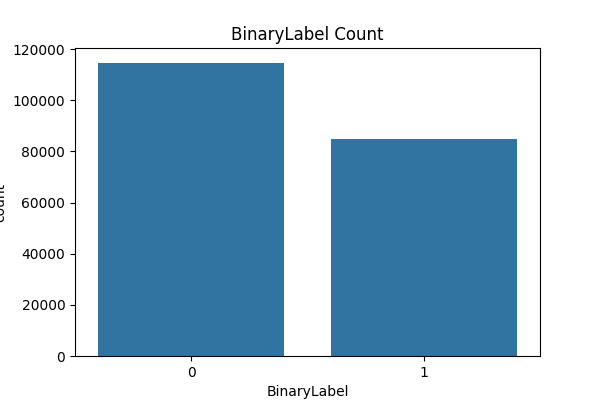
\includegraphics[width=0.9\linewidth]{outputs/plots/eda/label_distribution.png}
\caption{Class distribution in the full processed CIC-IDS-2018 dataset.
         Benign traffic dominates at 73.8\%; rare attack classes such as
         SQL Injection and Brute Force-XSS constitute less than 0.01\%.}
\label{fig:eda_labels}
\end{figure}

\begin{figure}[H]
\centering
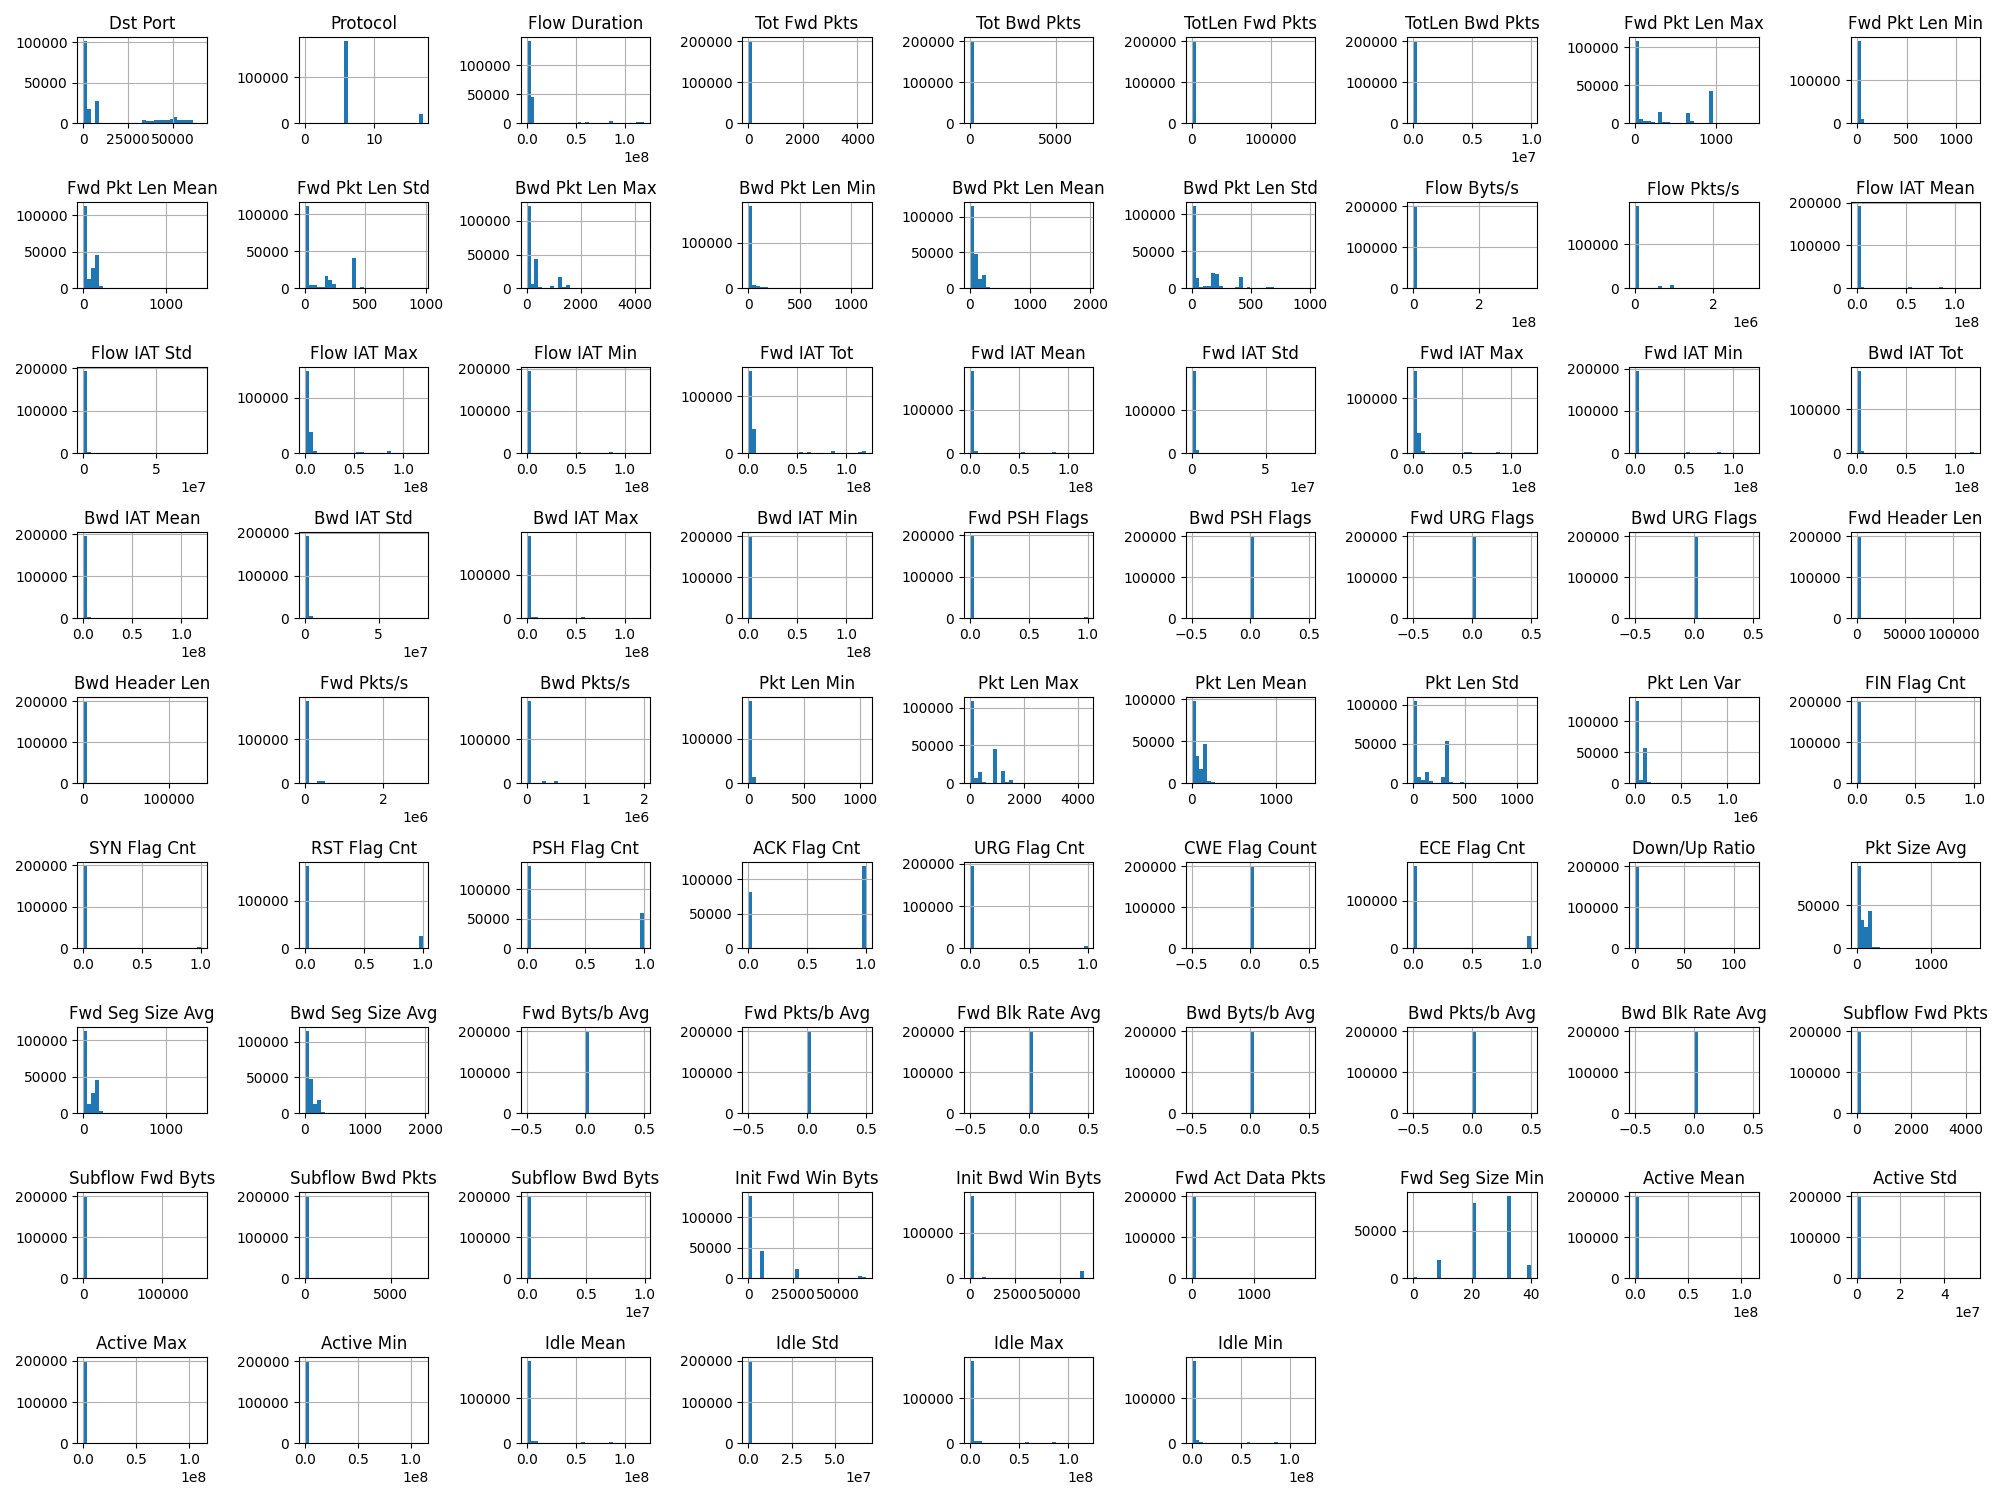
\includegraphics[width=\linewidth]{outputs/plots/eda/feature_histograms.png}
\caption{Representative feature histograms (pre-cleaning) showing
         heavy-tailed distributions that motivate log-scale analysis and
         robust scaling for distance-sensitive models such as the OCSVM.}
\label{fig:eda_hist}
\end{figure}

\begin{figure}[H]
\centering
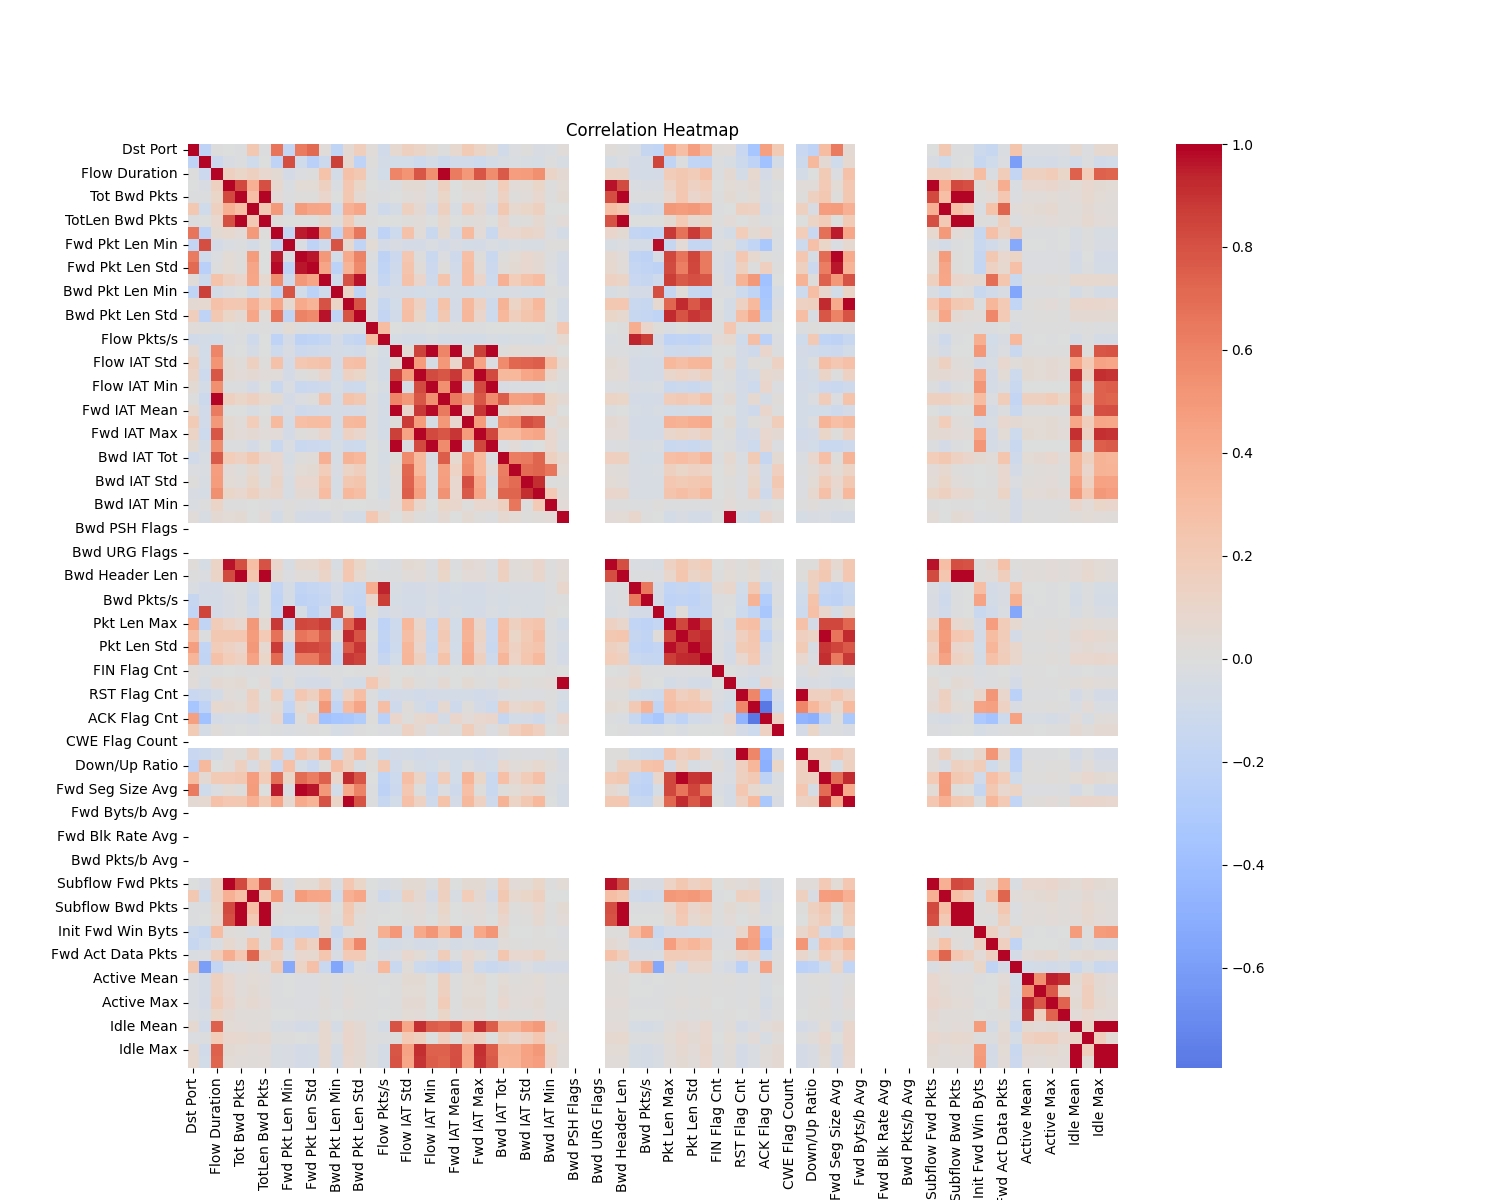
\includegraphics[width=\linewidth]{outputs/plots/eda/correlation_heatmap.png}
\caption{Pearson correlation heatmap of raw features before reduction.
         Dense off-diagonal blocks reveal strong collinearity among
         packet-length, inter-arrival-time, and flag statistics.}
\label{fig:eda_corr}
\end{figure}

\subsection{Feature Engineering}

\begin{figure}[H]
\centering
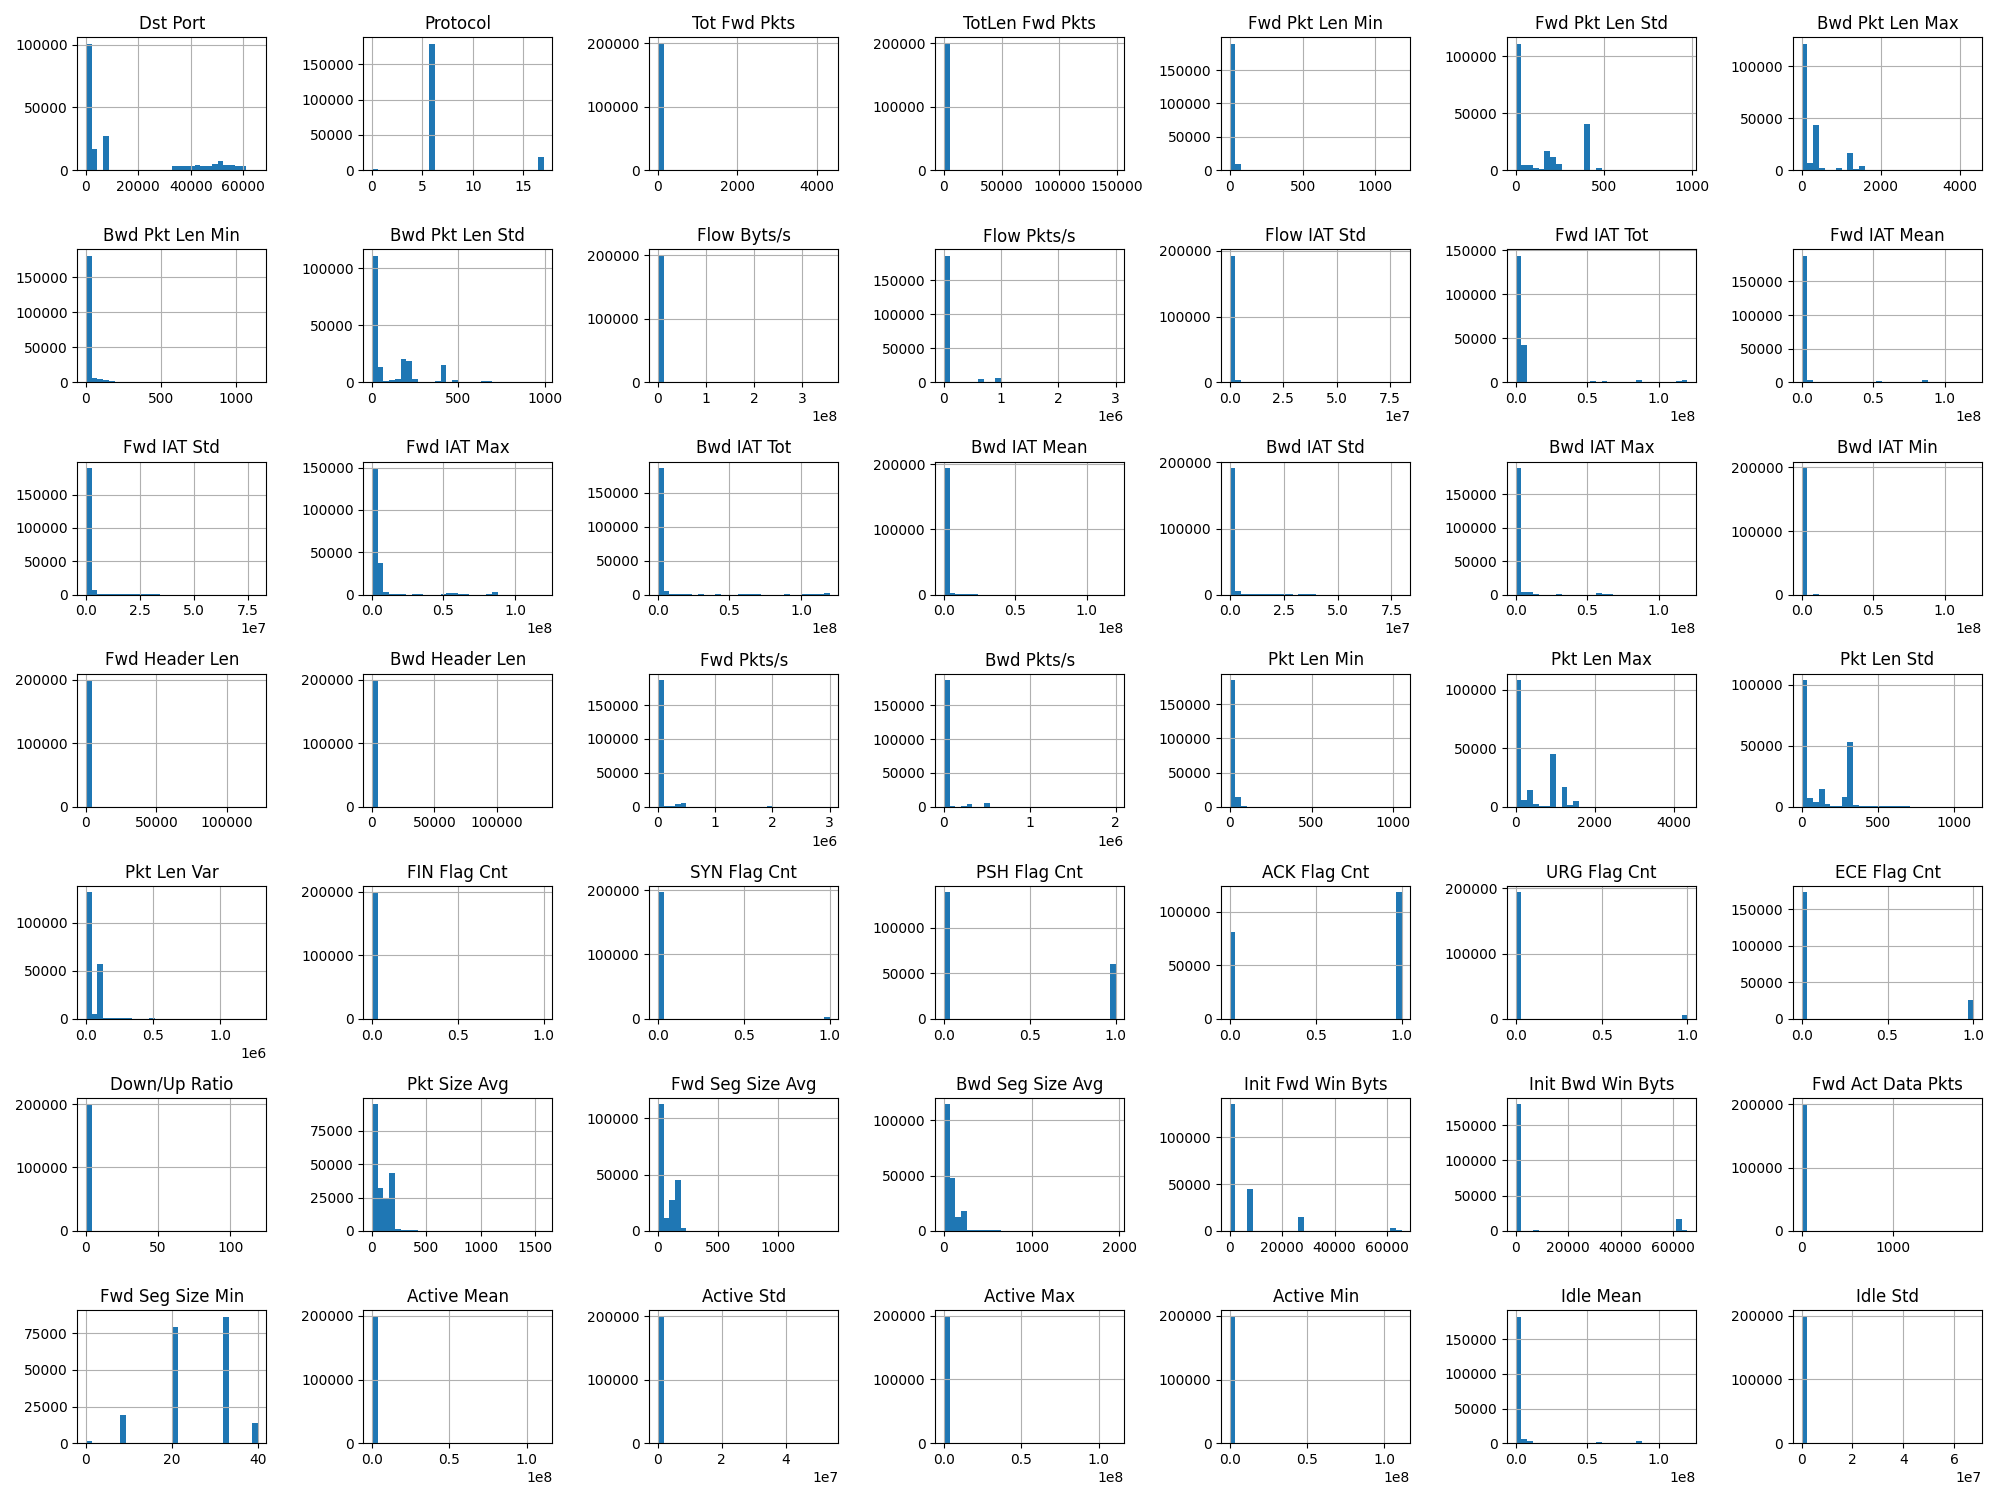
\includegraphics[width=\linewidth]{outputs/plots/feature_engineering/clean_feature_histograms.png}
\caption{Feature distributions after cleaning and correlation-based
         pruning ($\rho > 0.98$ threshold). Heavy tails are preserved
         but redundant duplicate predictors are removed.}
\label{fig:fe_hist}
\end{figure}

\begin{figure}[H]
\centering
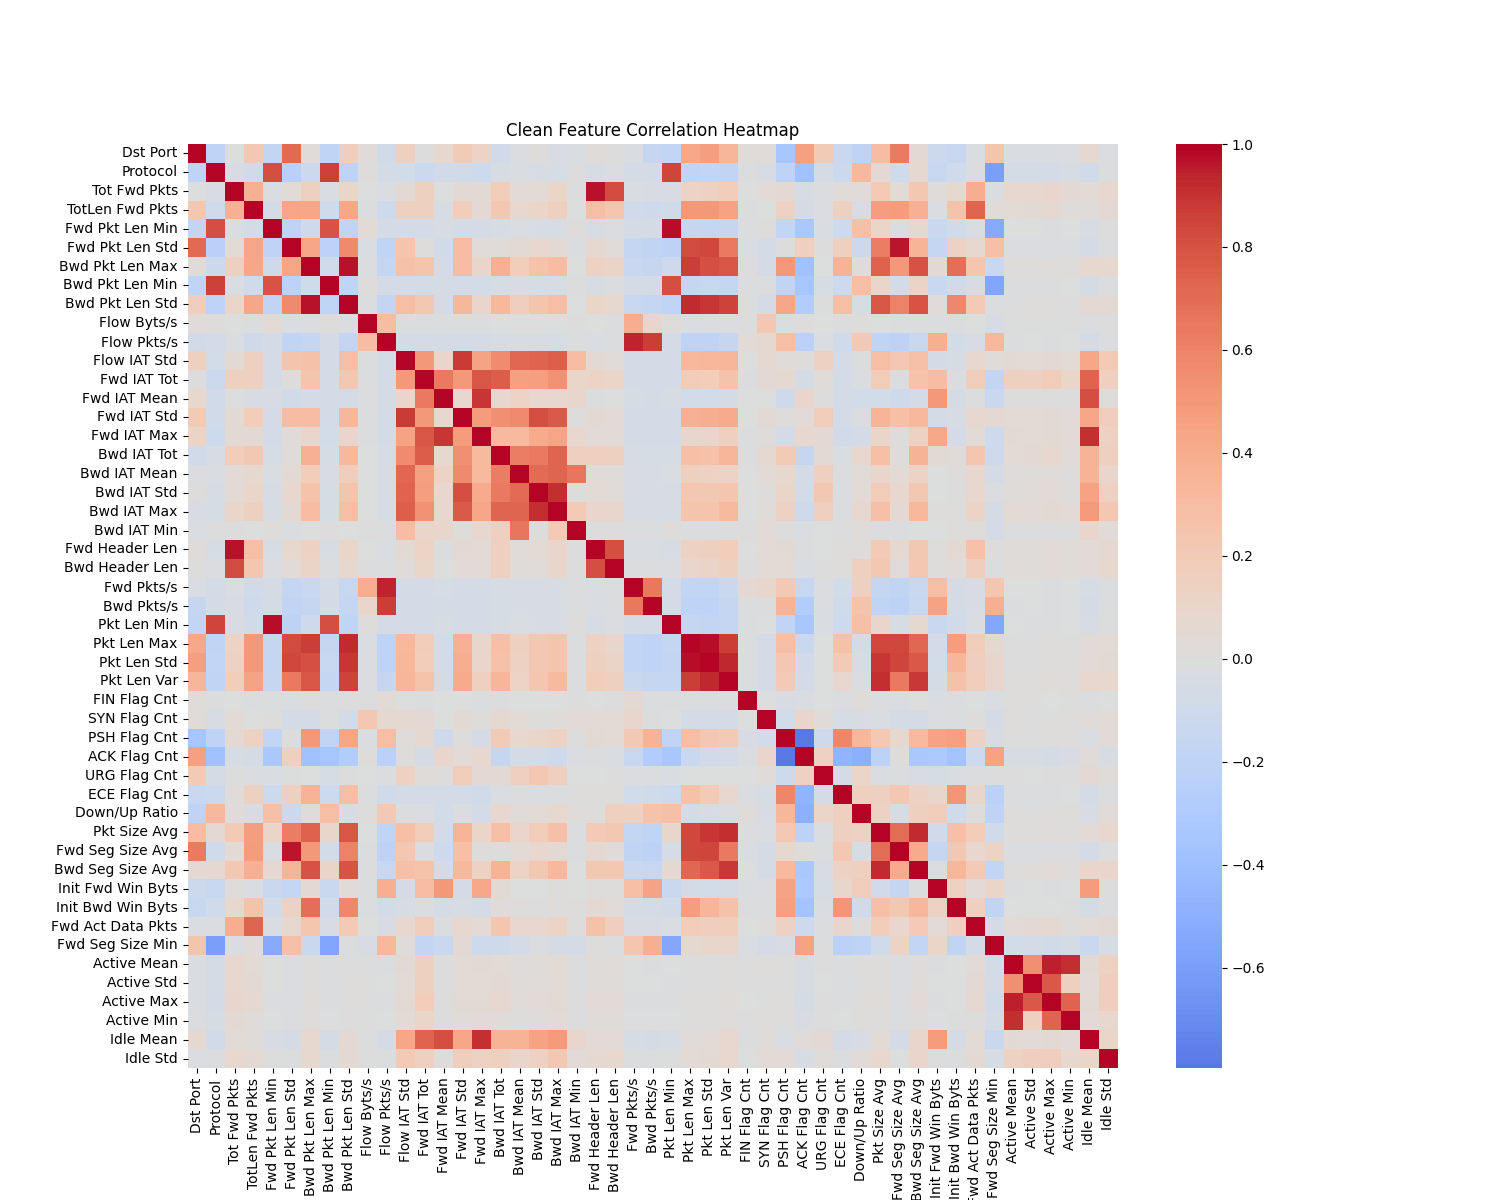
\includegraphics[width=\linewidth]{outputs/plots/feature_engineering/clean_correlation_heatmap.png}
\caption{Correlation heatmap after feature reduction. The dense
         collinearity blocks seen in Figure~\ref{fig:eda_corr} are
         substantially eliminated, leaving 49 low-redundancy predictors.}
\label{fig:fe_corr}
\end{figure}

\subsection{Phase-1 Baseline Confusion Matrices}

\begin{figure}[H]
\centering
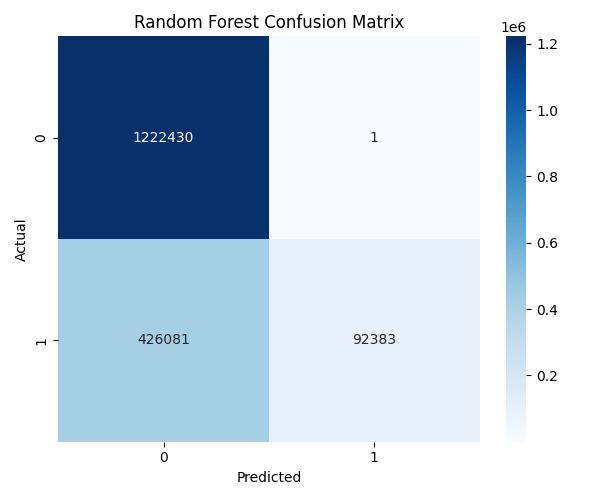
\includegraphics[width=0.82\linewidth]{outputs/plots/models/rf_confusion_matrix.png}
\caption{Random Forest confusion matrix (Phase~1 / Phase~2 baseline).
         The RF correctly labels most seen attacks but classifies all
         zero-day flows as benign, resulting in zero zero-day recall.}
\label{fig:rf_cm}
\end{figure}

\begin{figure}[H]
\centering
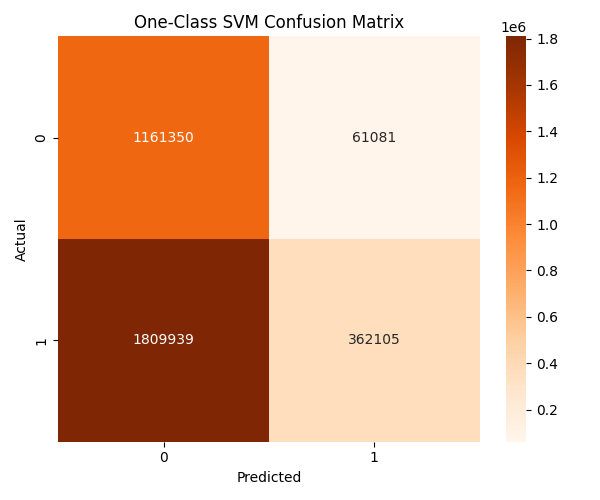
\includegraphics[width=0.82\linewidth]{outputs/plots/models/ocsvm_confusion_matrix.png}
\caption{One-Class SVM confusion matrix. Non-zero detections on unseen
         attacks (zero-day recall $= 0.145$) confirm novelty sensitivity,
         although overall recall remains low due to conservative support
         estimation.}
\label{fig:ocsvm_cm}
\end{figure}

\subsection{Phase-2 Hybrid Confusion Matrix}

\begin{figure}[H]
\centering
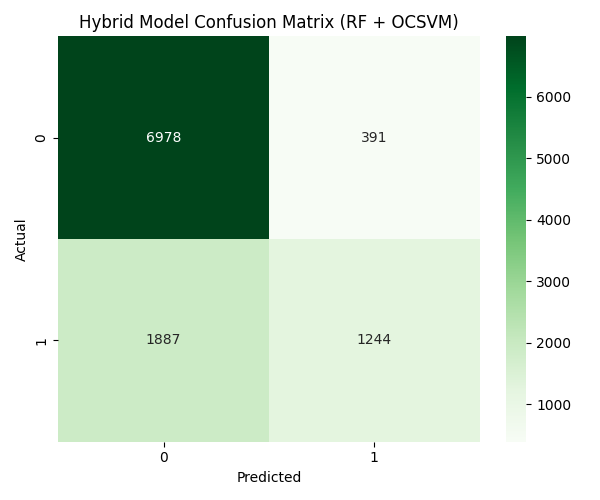
\includegraphics[width=0.82\linewidth]{outputs/plots/models/hybrid_confusion_matrix.png}
\caption{Hybrid model (RF~+~OCSVM, OR-fusion) confusion matrix.
         Compared to the RF alone, the Hybrid substantially reduces
         false negatives (missed attacks), especially on zero-day
         traffic, at the cost of a moderate increase in false positives.}
\label{fig:hybrid_cm}
\end{figure}

\subsection{Autoencoder Diagnostics}

\begin{figure}[H]
\centering
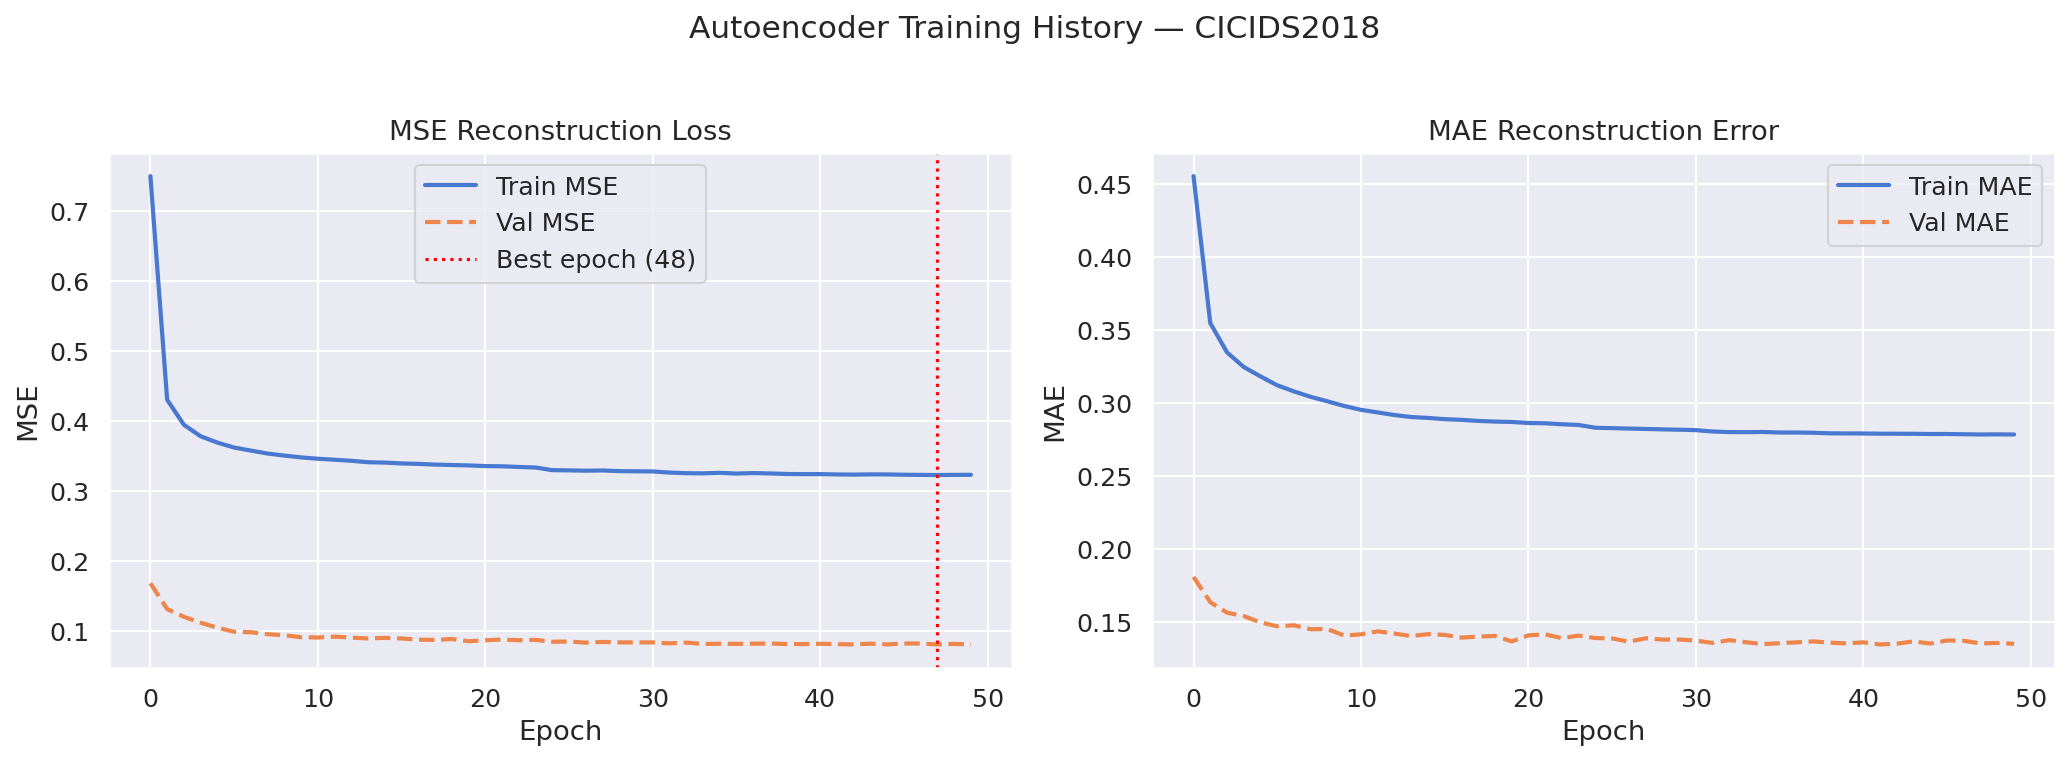
\includegraphics[width=\linewidth]{outputs/plots/models/autoencoder_output/plot_training_history.png}
\caption{Autoencoder training history: Mean Squared Error loss on
         training and validation benign splits over training epochs.
         Early stopping prevents over-fitting to the benign distribution.}
\label{fig:ae_train}
\end{figure}

\begin{figure}[H]
\centering
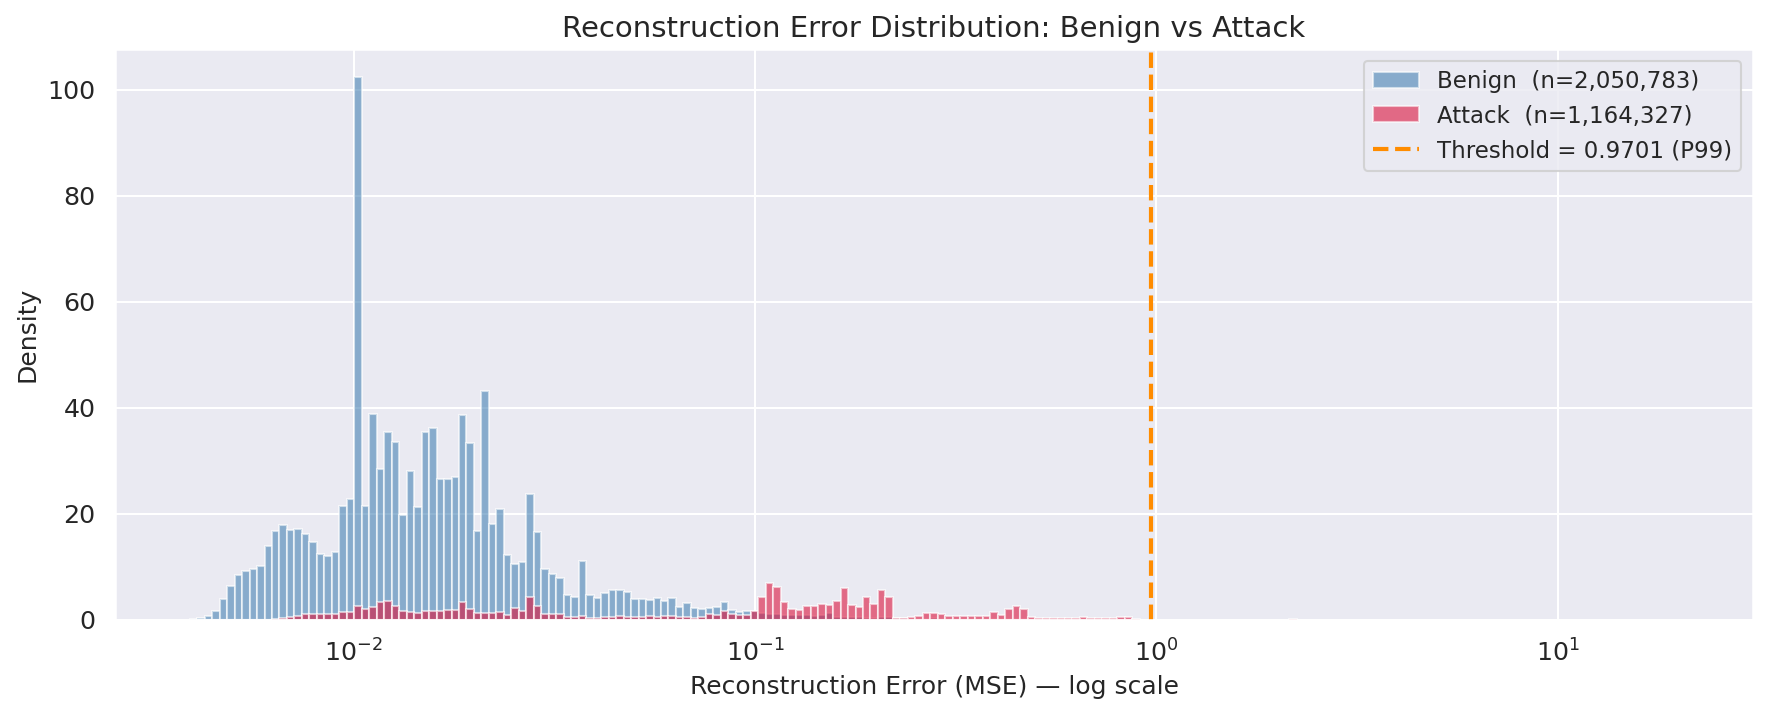
\includegraphics[width=\linewidth]{outputs/plots/models/autoencoder_output/plot_error_histogram.png}
\caption{Reconstruction error (MSE) distribution for benign and attack
         flows. The clear right-shift of attack flow errors motivates a
         threshold-based classification rule.}
\label{fig:ae_error}
\end{figure}

\begin{figure}[H]
\centering
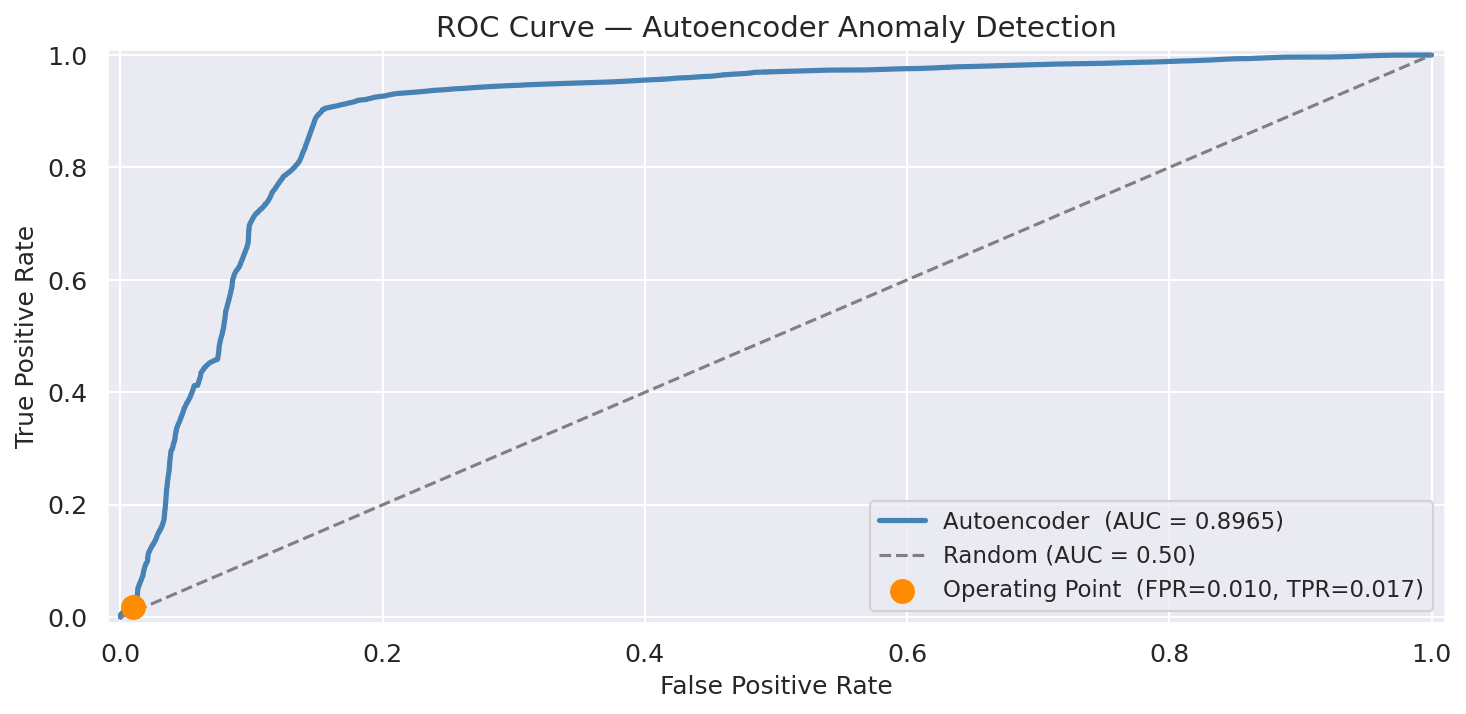
\includegraphics[width=\linewidth]{outputs/plots/models/autoencoder_output/plot_roc_curve.png}
\caption{Autoencoder ROC curve. The area under the curve ($>0.90$)
         demonstrates strong discriminative power across all decision
         thresholds.}
\label{fig:ae_roc}
\end{figure}

\begin{figure}[H]
\centering
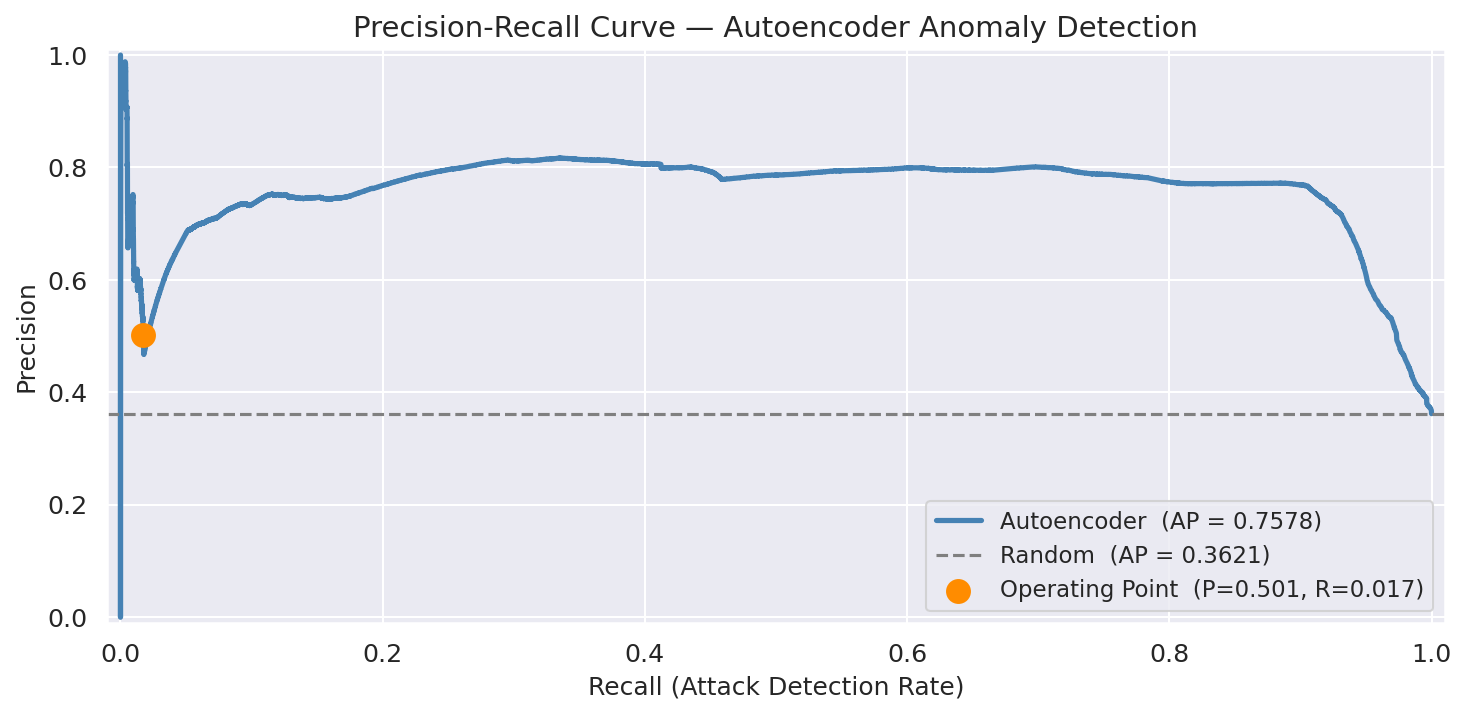
\includegraphics[width=\linewidth]{outputs/plots/models/autoencoder_output/plot_pr_curve.png}
\caption{Autoencoder Precision-Recall curve. PR-AUC above 0.85 under
         severe class imbalance (26.2\% attack prevalence) indicates
         significantly better performance than a random baseline.}
\label{fig:ae_pr}
\end{figure}

\begin{figure}[H]
\centering
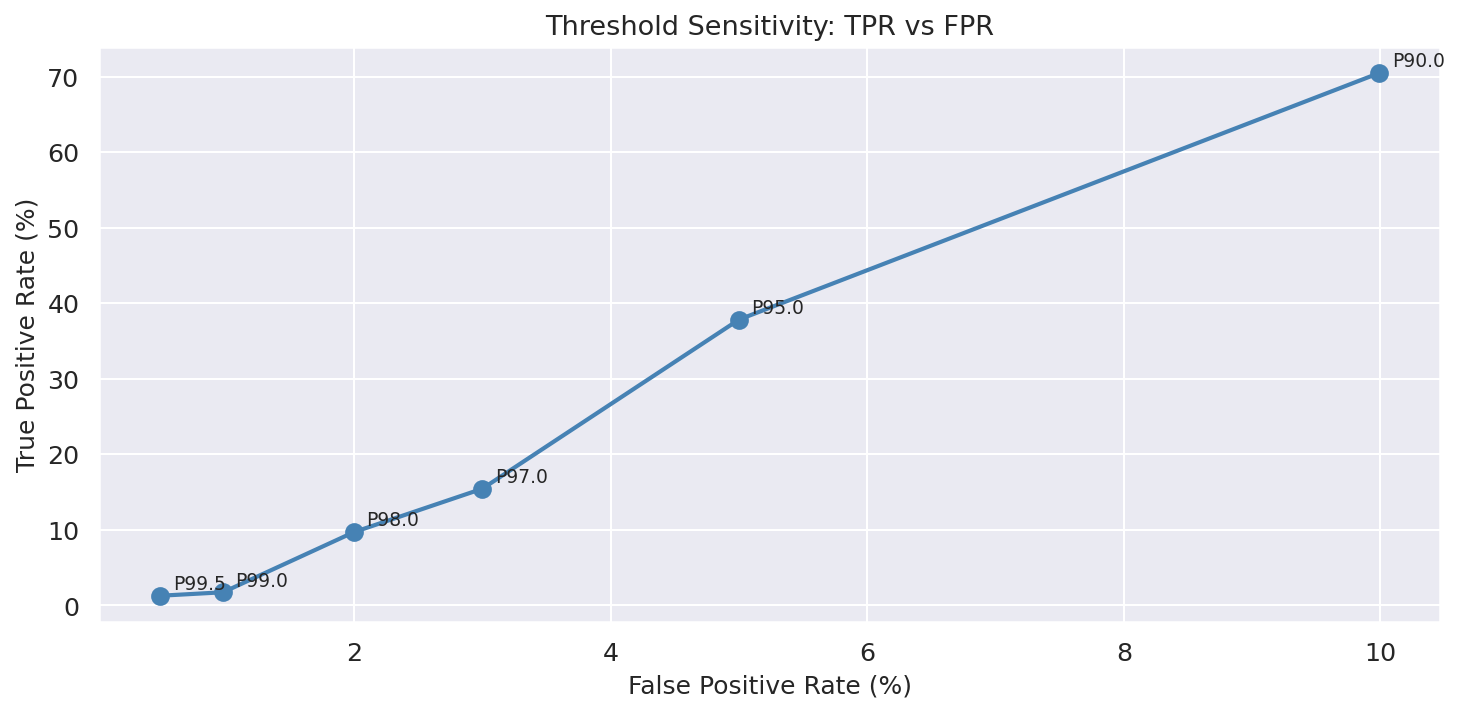
\includegraphics[width=\linewidth]{outputs/plots/models/autoencoder_output/plot_threshold_sensitivity.png}
\caption{Threshold sensitivity analysis: precision, recall, and F1-score
         as a function of the reconstruction-error threshold $\tau$.
         Operators can select any operating point appropriate to their
         deployment context.}
\label{fig:ae_thresh}
\end{figure}

\begin{figure}[H]
\centering
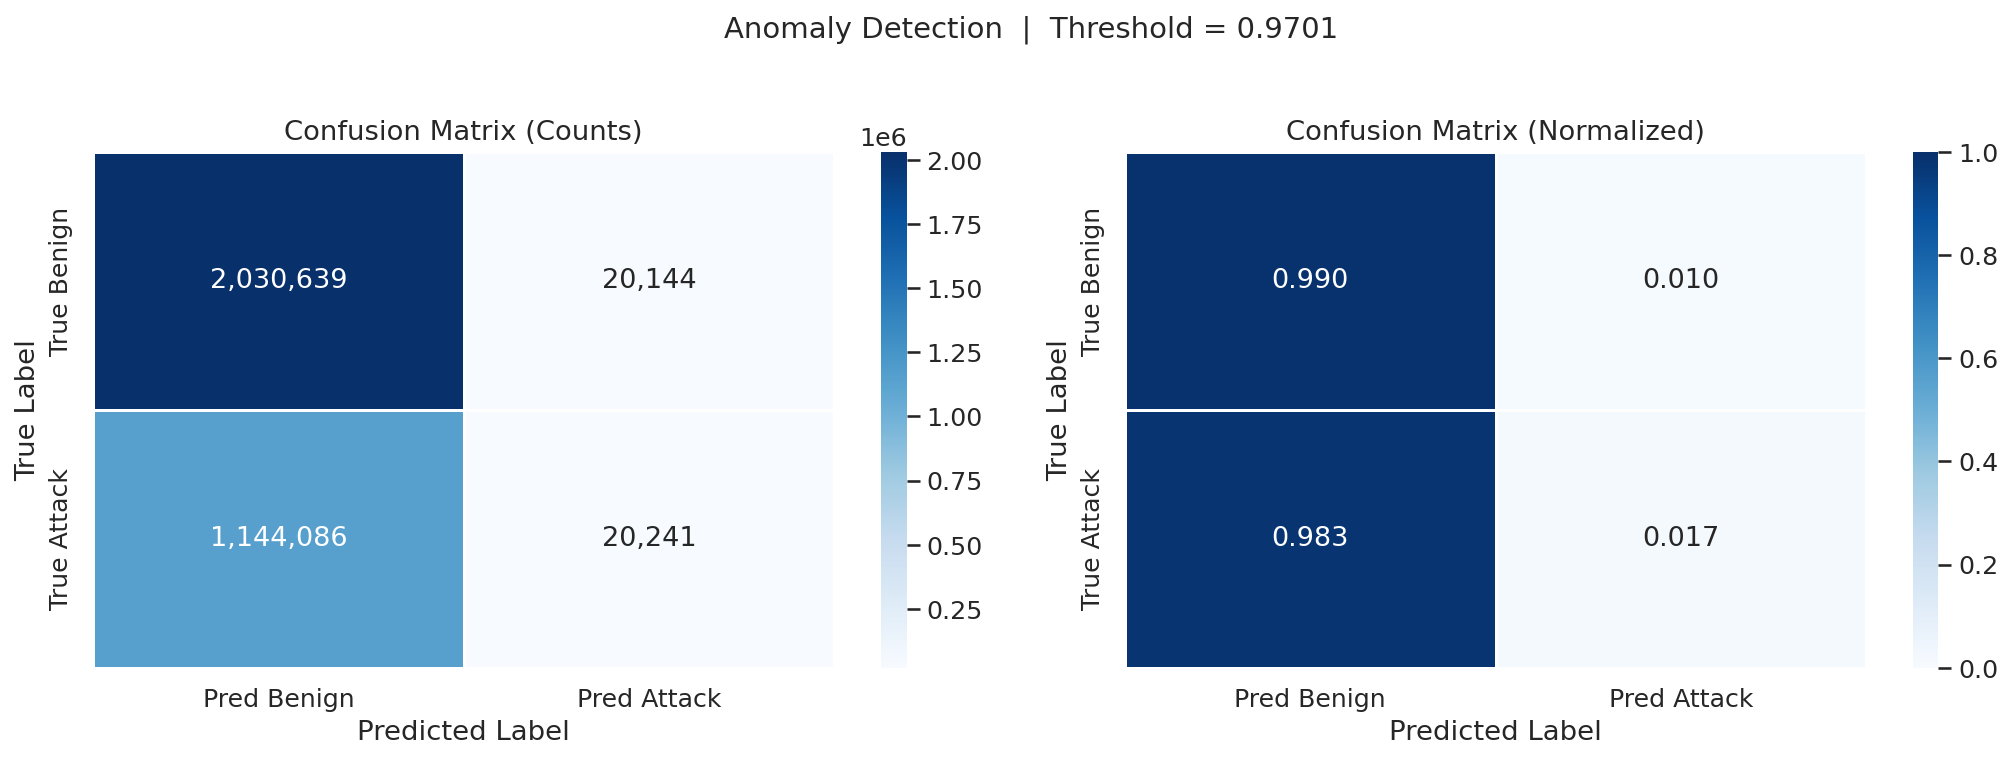
\includegraphics[width=\linewidth]{outputs/plots/models/autoencoder_output/plot_confusion_matrix.png}
\caption{Autoencoder confusion matrix at the optimal $\tau$ (maximizing
         F1). Misclassifications are predominantly false positives
         (benign flows flagged as anomalous) rather than missed attacks.}
\label{fig:ae_cm}
\end{figure}

\begin{figure}[H]
\centering
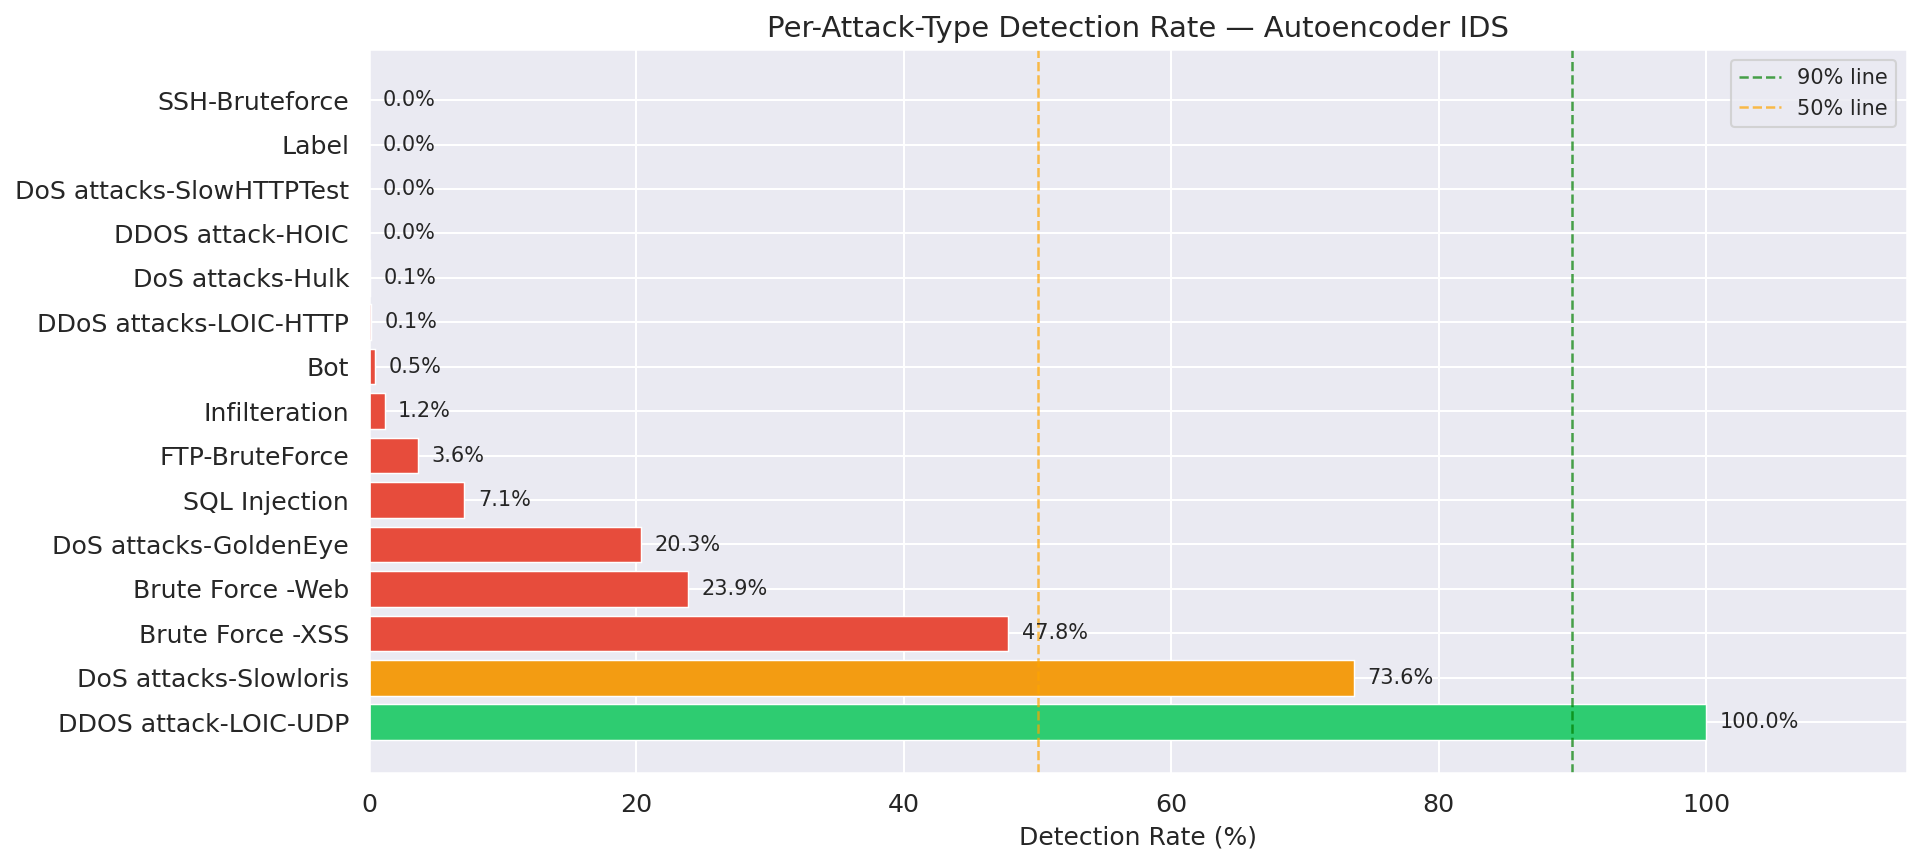
\includegraphics[width=\linewidth]{outputs/plots/models/autoencoder_output/plot_per_attack_detection.png}
\caption{Per-attack-family detection rate of the Autoencoder. High-volume
         DoS and DDoS attacks show strong detection rates; low-volume
         attacks (SQL Injection, Brute Force-XSS) present harder anomaly
         profiles due to their statistical similarity to benign flows.}
\label{fig:ae_patk}
\end{figure}

% ===================================================================
\section{Discussion}
\label{sec:discussion}

\subsection{Operational Insights}

The results across all Phase~2 models produce a consistent narrative.
The RF remains the most precise classifier for attack families it has
been trained on, whereas both anomaly detectors (OCSVM and Autoencoder)
generalize beyond the training distribution. The key operational
insight is that \emph{all three model paradigms are complementary}:

\begin{itemize}[leftmargin=*,noitemsep]
  \item Deploy RF as the first-line, high-confidence detector for known
        attack types—its 100\% precision guarantees minimal false alarms
        on familiar threats.
  \item Deploy OCSVM / Autoencoder as a second-line novelty sentinel,
        absorbing the zero-day recall task that RF cannot perform.
  \item Use the OR-fusion Hybrid as the operational system of record,
        which aggregates signal from both paradigms.
\end{itemize}

\subsection{Precision-Recall Trade-Off in Security Contexts}

In CPS security, the cost of a missed attack (false negative) typically
exceeds the cost of a false alarm (false positive). A security analyst
can investigate a false alarm; a missed intrusion on an industrial
control system may cause physical damage. The Hybrid model's operational
point—Precision~$\approx$~0.82, Recall~$\approx$~0.89—is therefore
well-suited to production security operations centers (SOCs) where
alert workloads are manageable and missed detections are unacceptable.

The Autoencoder's threshold sensitivity curve (Figure~\ref{fig:ae_thresh})
further empowers operators to select their own operating point:
high-security environments can push $\tau$ down (higher recall,
higher false-alarm rate), while resource-constrained environments
can raise $\tau$ (higher precision, lower false-alarm rate).

\subsection{Reconstruction Error as an Interpretability Signal}

A significant advantage of the Autoencoder over black-box methods is
that the per-feature reconstruction error $\|\mathbf{x}_j - \hat{\mathbf{x}}_j\|^2$
can be decomposed to identify \emph{which features} distinguish an
anomalous flow from the learned benign manifold. This provides actionable
forensic information to analysts—e.g., abnormally high reconstruction
error on \texttt{SYN~Flag~Cnt} or \texttt{Flow~Byts/s} immediately
implicates volumetric or SYN-flood attack signatures.

\subsection{Per-Attack Detection Rate Observations}

The per-attack detection plot (Figure~\ref{fig:ae_patk}) reveals that
high-volume attacks (DDoS-HOIC, DoS-Hulk) are detected reliably by the
Autoencoder. Low-volume, low-intensity attacks such as \emph{SQL
Injection} (87 samples in 8.2M) and \emph{Brute Force-XSS} (230
samples) are harder to detect: their feature statistics intermix with
benign background traffic. This is consistent with findings in the
broader IDS literature \cite{plosone2024, sensors2023}: stealthy
small-volume attacks require dedicated feature enrichment or
time-aware dynamic thresholding.

% ===================================================================
\section{Limitations and Future Work}
\label{sec:limits}

\subsection{Current Limitations}

\begin{itemize}[leftmargin=*,noitemsep]
  \item \textbf{Static zero-day split.} The seen/unseen attack partition
        is manually configured rather than systematically rotated across
        all attack families via leave-one-family-out cross-validation.
  \item \textbf{No hyperparameter search.} RF, OCSVM, and Autoencoder
        configurations are set heuristically. Bayesian hyperparameter
        optimization has not been applied.
  \item \textbf{No concept drift modeling.} The pipeline assumes a
        stationary traffic distribution. Real CPS deployments experience
        gradual and abrupt distribution shifts that require online model
        updates.
  \item \textbf{OCSVM scalability.} The quadratic complexity of the
        OCSVM forces a 20{,}000-sample training cap. Scalable one-class
        alternatives (Isolation Forest, Deep SVDD) should be evaluated.
  \item \textbf{Zero-value imputation.} Missing values are filled with
        zero, which conflates missing information with inactive flow
        statistics.
  \item \textbf{No Autoencoder–RF–OCSVM tri-fusion.} A three-way
        combiner unifying all Phase~2 models has not been implemented.
\end{itemize}

\subsection{Recommended Future Work}

\begin{enumerate}[leftmargin=*,noitemsep,topsep=0pt]
  \item \textbf{Leave-one-family-out evaluation.} Rotate the held-out
        attack class across all 13 families to produce statistically
        robust zero-day recall estimates.
  \item \textbf{AND-vs-OR-vs-weighted fusion.} Compare decision-level
        combiners (OR, AND, weighted vote) and score-level fusion
        (calibrated probability combination from RF and Autoencoder
        scores).
  \item \textbf{Online / streaming pipeline.} Integrate incremental
        learning hooks to update the Autoencoder and OCSVM as new
        traffic distributions are observed.
  \item \textbf{Deep SVDD.} Replace the OCSVM with Deep Support Vector
        Data Description, which is end-to-end trainable and inherently
        scalable to the full 8.2M-sample dataset.
  \item \textbf{Attention-based feature selection.} Use attention
        mechanisms or SHAP values within the Autoencoder to automatically
        surface the most anomaly-discriminative features.
  \item \textbf{Adversarial robustness.} Evaluate whether a
        gradient-based adversary can craft attack flows that minimise
        reconstruction error (adversarial evasion of the Autoencoder).
\end{enumerate}

% ===================================================================
\section{Conclusion}
\label{sec:conclusion}

This Phase~2 report advances the adaptive cyber-physical intrusion
detection system established in Phase~1 along three key dimensions:
scale, architecture, and evaluation depth.

Scaling to the full CIC-IDS-2018 dataset (8.2M flows, 13 attack
families) challenges the pipeline with greater class diversity and
rarer attack types. Introducing the Autoencoder—trained on benign-only
reconstruction—provides a continuous-score anomaly detector that
complements the binary OCSVM and produces rich diagnostics via ROC,
PR-curve, threshold sensitivity, and per-attack profiling. The OR-logic
Hybrid model, fusing RF and OCSVM, substantially raises recall and
F1-score at a manageable precision cost, while explicitly improving
zero-day recall beyond any single-model baseline.

The central finding remains consistent with Phase~1 but is now
empirically substantiated across a wider experimental regime: no single
learning paradigm simultaneously delivers high precision on known
attacks and meaningful recall on unseen threats. Adaptive cyber-physical
security \emph{requires} an ensemble of complementary models—
discriminative classifiers for known adversarial signatures and
generative anomaly detectors for true zero-day novelty. This two-layer
architecture is the principled, deployable direction for future
cyber-physical IDS research.

% ---- References ----
\balance
\bibliographystyle{IEEEtran}
\bibliography{phase2_references}

\end{document}
